% !TeX root = ../pres.tex

\section{Bohr'sches Magneton}
  \subsection{Hysterese Effekt}
    \begin{myframe}{\subsecname}
      \begin{itemize}
        \item Magnetfeldmessung bei 6 Stromstärken zwischen 8 und 13A
        \item für fallende und steigende Stromstärke
        \item Ermittlung des Zusammenhangs zwischen Stromstärke und Magnetfeld
      \end{itemize}

      Resultat:
      \begin{align}
        m_u = \inclineUp\\
        m_d = \inclineDown
      \end{align}

      $\Rightarrow$ Abweichung: < 1$\sigma$
    \end{myframe}

    \begin{myframe}{}
        \begin{figure}
          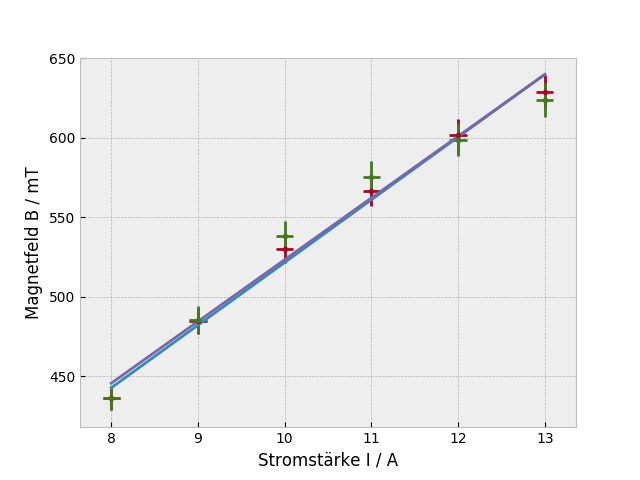
\includegraphics[height=.85\paperheight]{img/hysteresis.png}
          \caption{Hysterese}
          \label{Hysterese}
        \end{figure}
    \end{myframe}

  \subsection{Polarisation}
    \subsubsection{longitudinal}
      \begin{myframe}{\subsecname\ - \subsubsecname}
        \onslide<1,3>{
          \begin{itemize}
            \item mit und ohne linearem Polarisationsfilter: 2 Linien pro Beugungsordnung
            \item[$\rightarrow$] zirkulär polarisiert
            \item[]
            \item<3> mit $\lambda /4$-Filter in linear polarisiertes umwandeln
            \item<3> jetzt erhält man eine Linie pro Beugungsordnung, nach linearem Polarisationsfilter
            \item[$\rightarrow$]<3> Rotation des Linearfilters um 90° wechselt zwischen beiden Linien
          \end{itemize}
        }
        \onslide<2,4>{
          \vspace{-.35\paperheight}
        }
        \begin{figure}
          \centering
          \onslide<2>{
            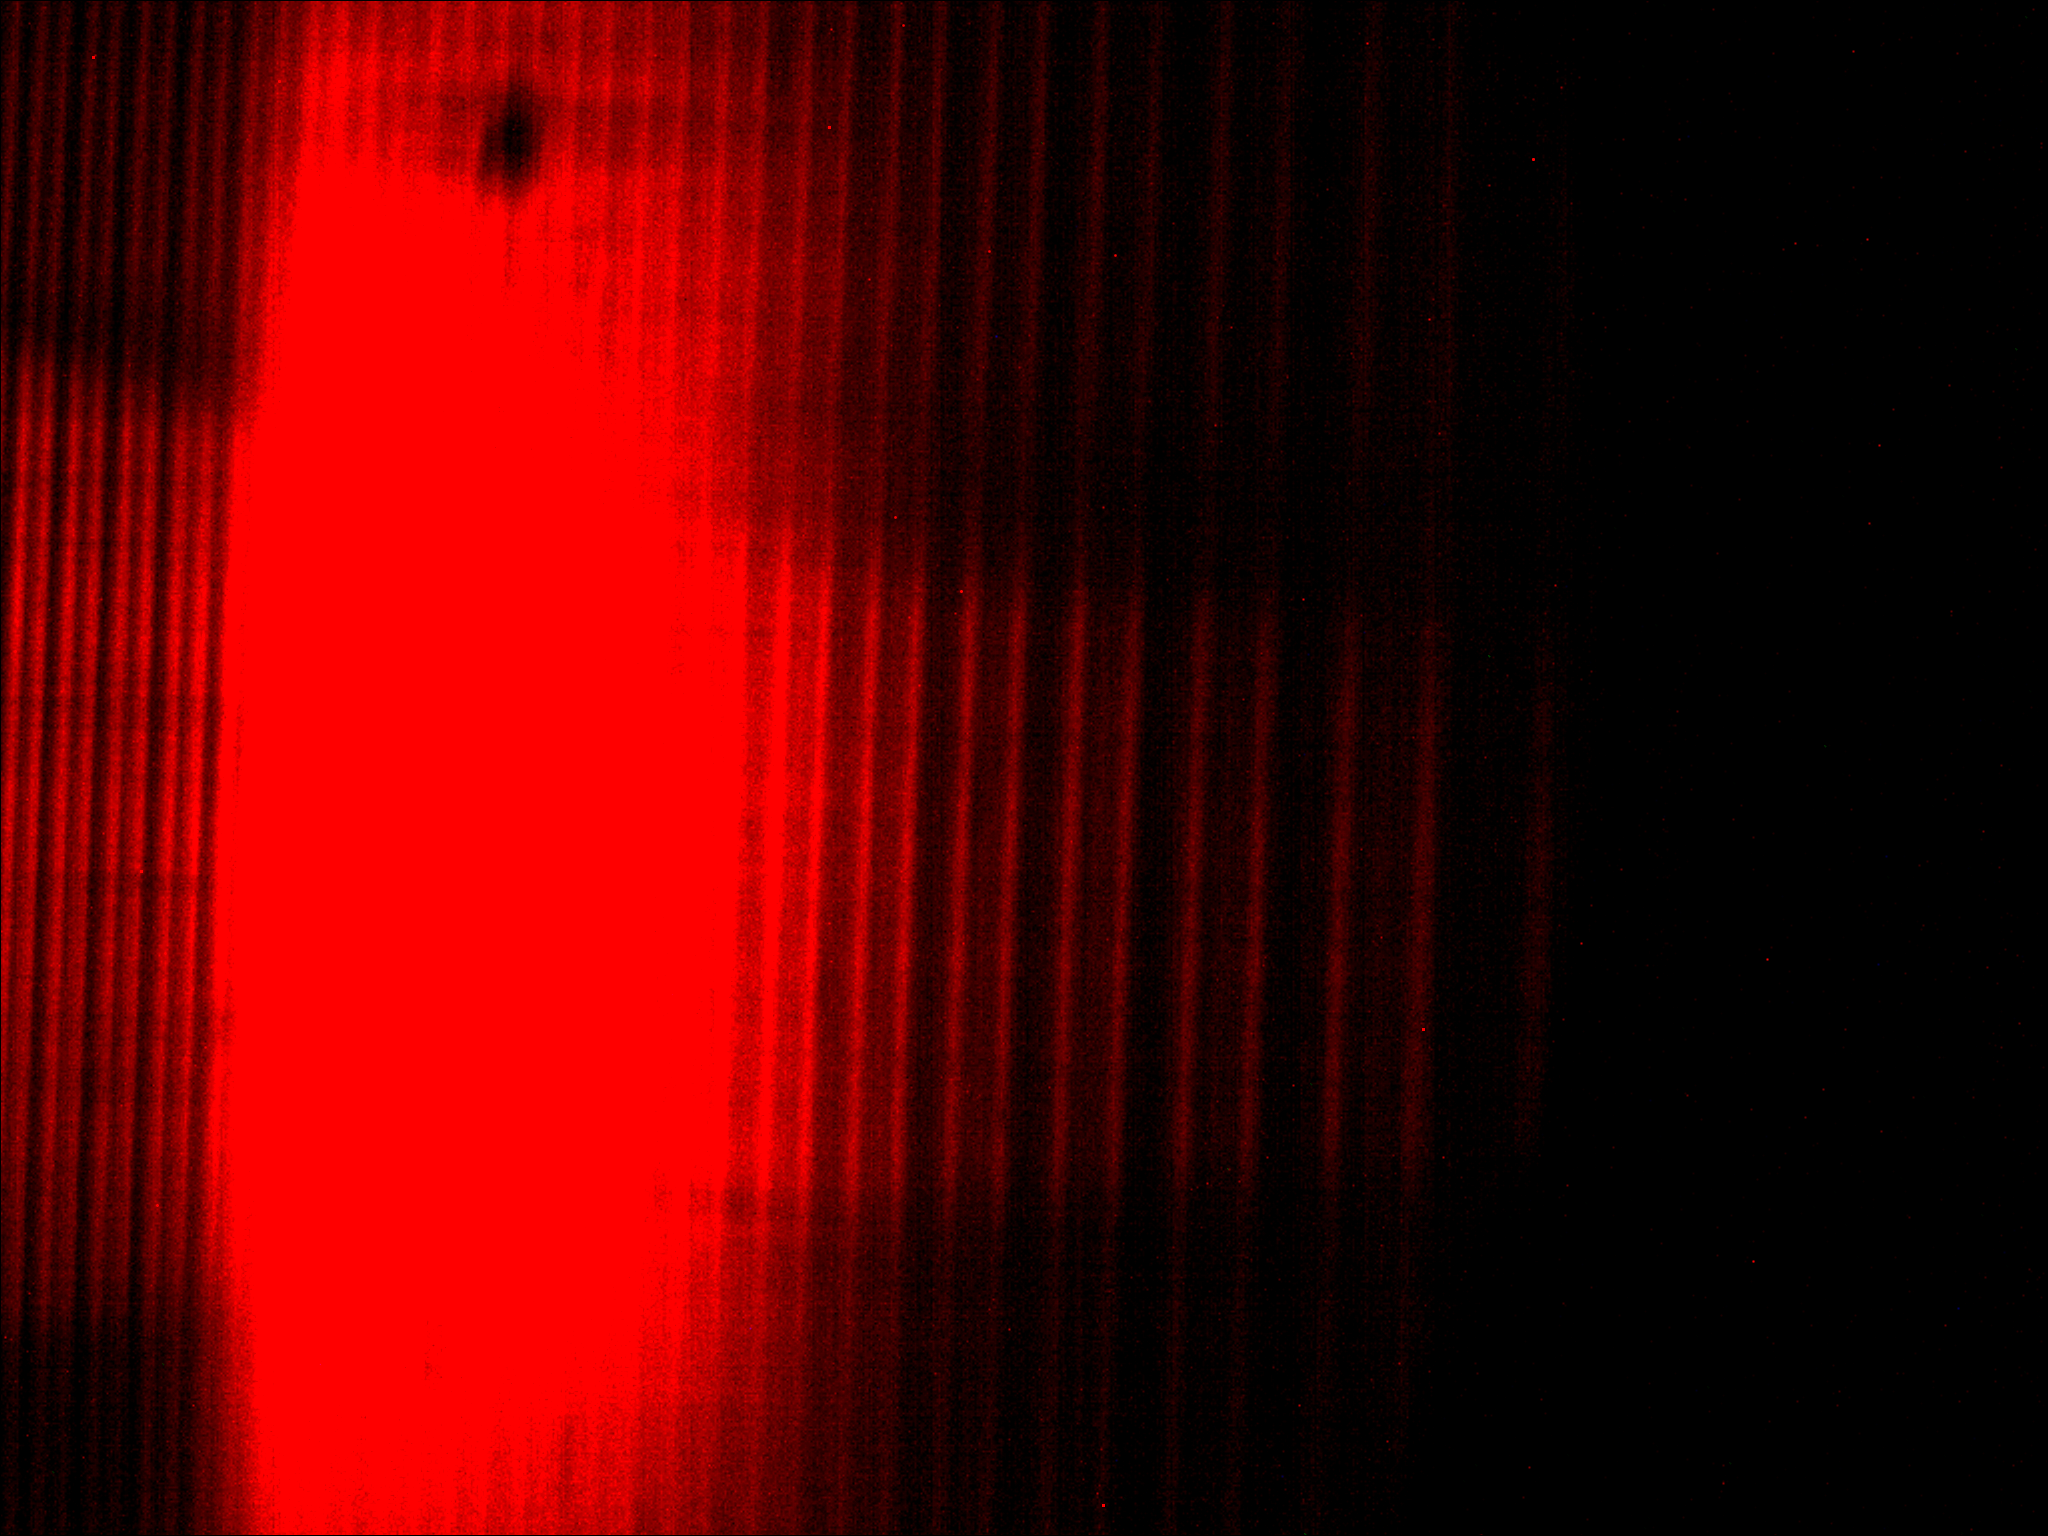
\includegraphics[height=.6\paperheight]{img/long_ohne.png}
            \caption{longitudinale Polarisation ohne Fiter}
            \label{long_ohne}
          }
          \onslide<4>{
            \vspace{-.75\paperheight}
            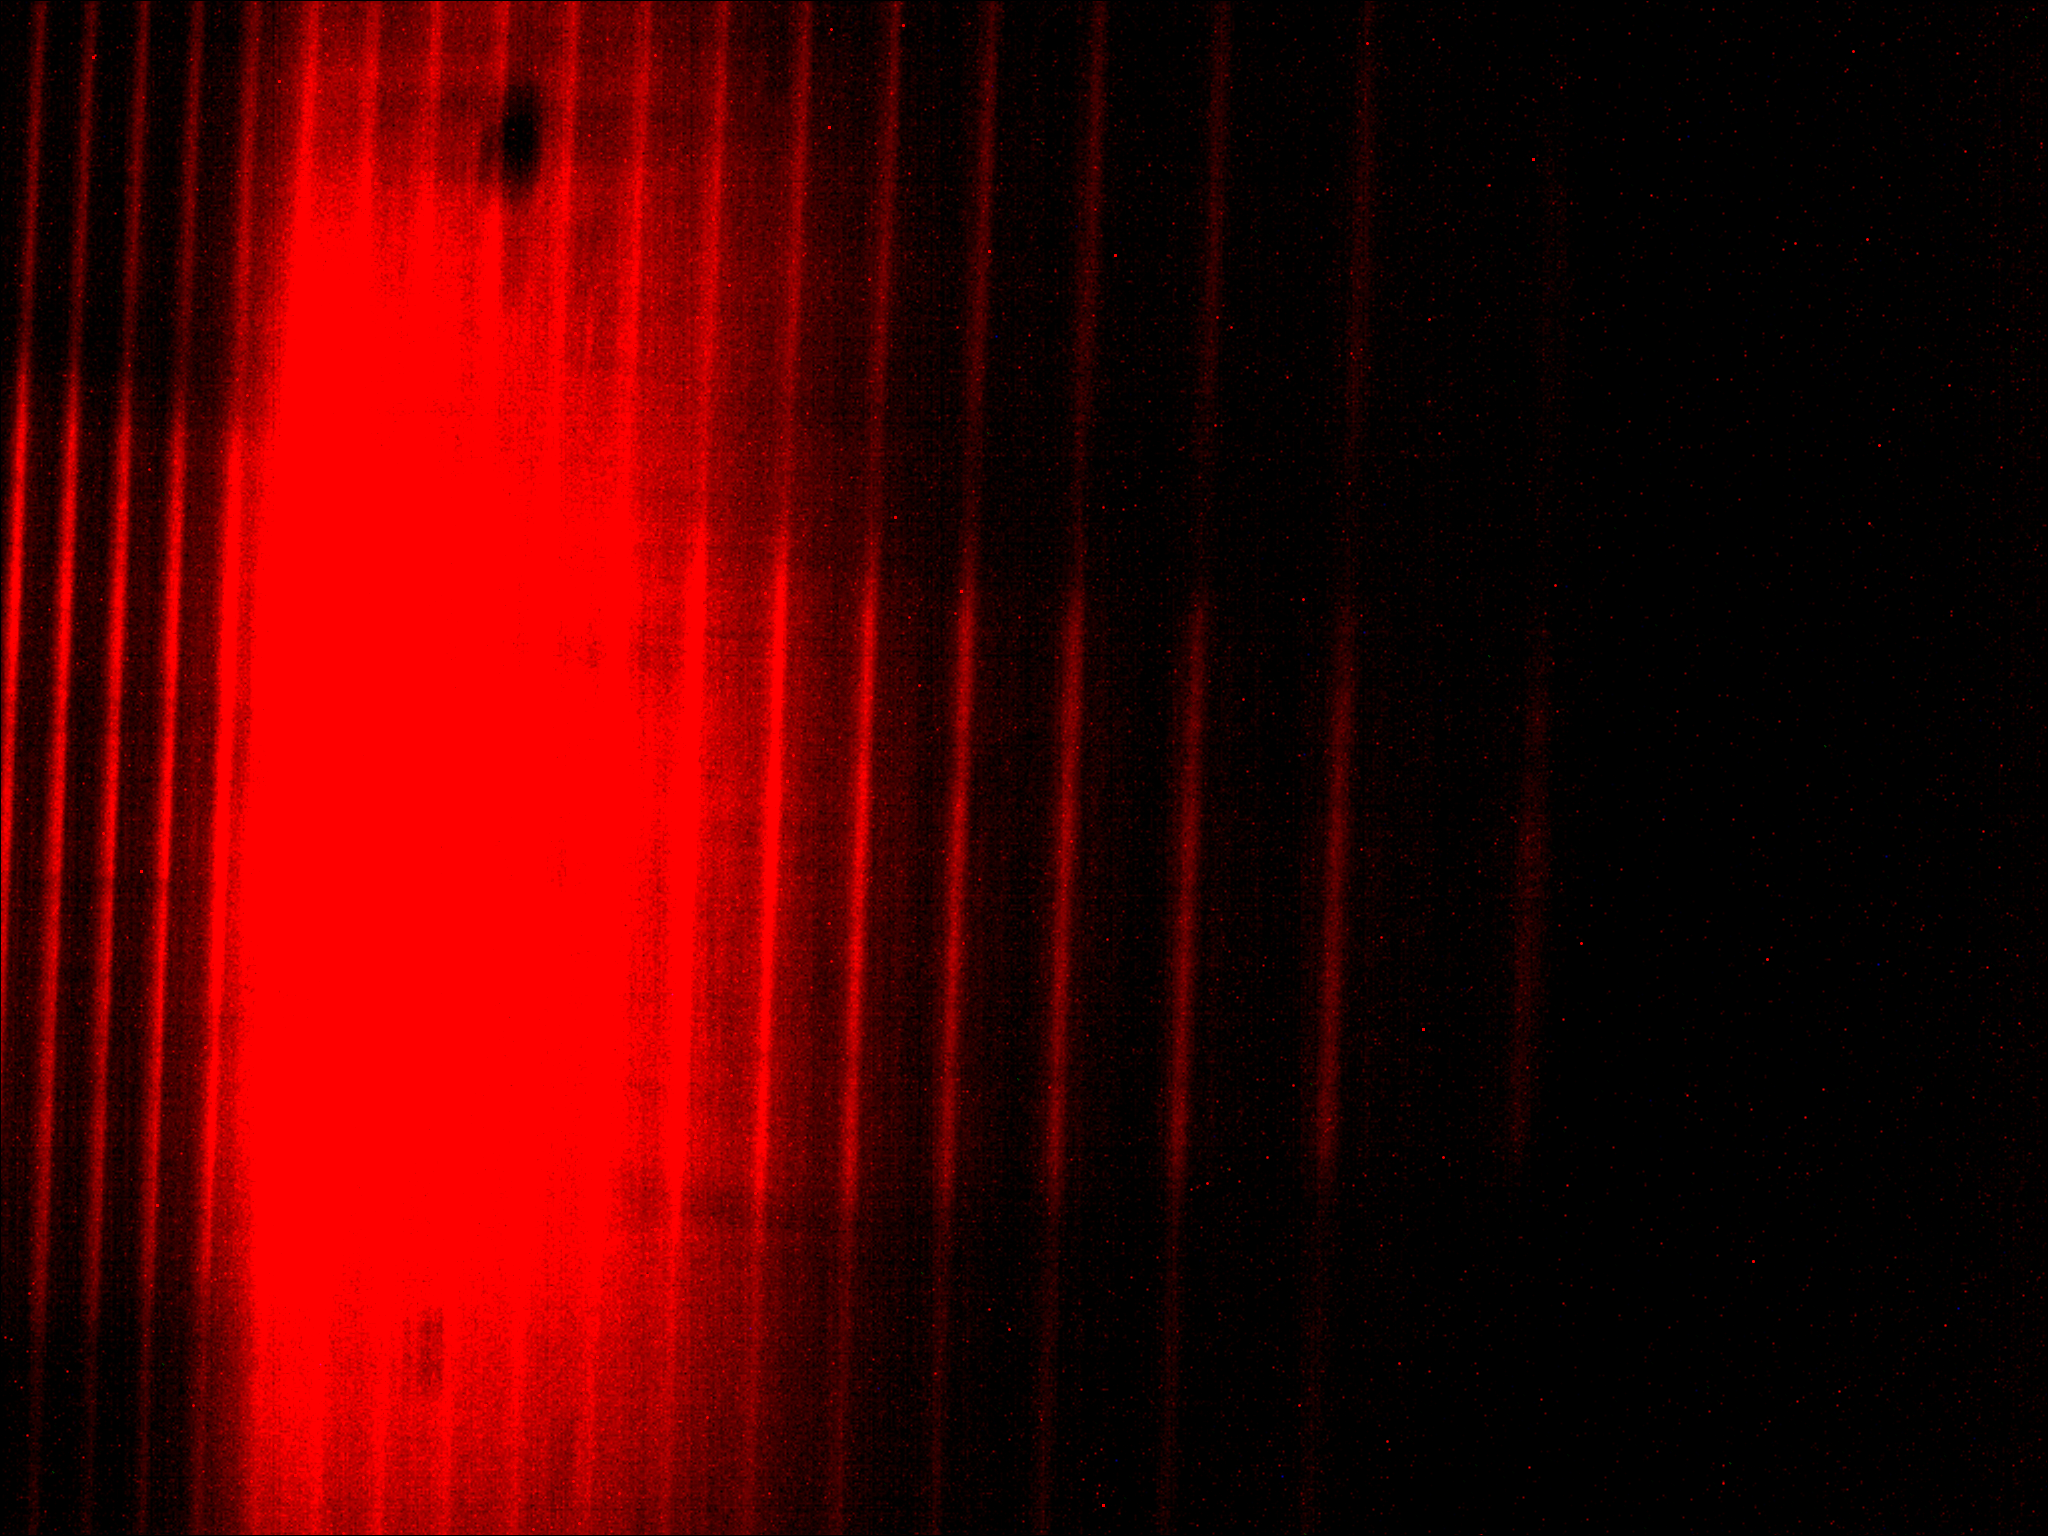
\includegraphics[width=.5\paperwidth, trim={0 650pt 0 200pt}, clip]{img/long_2}
            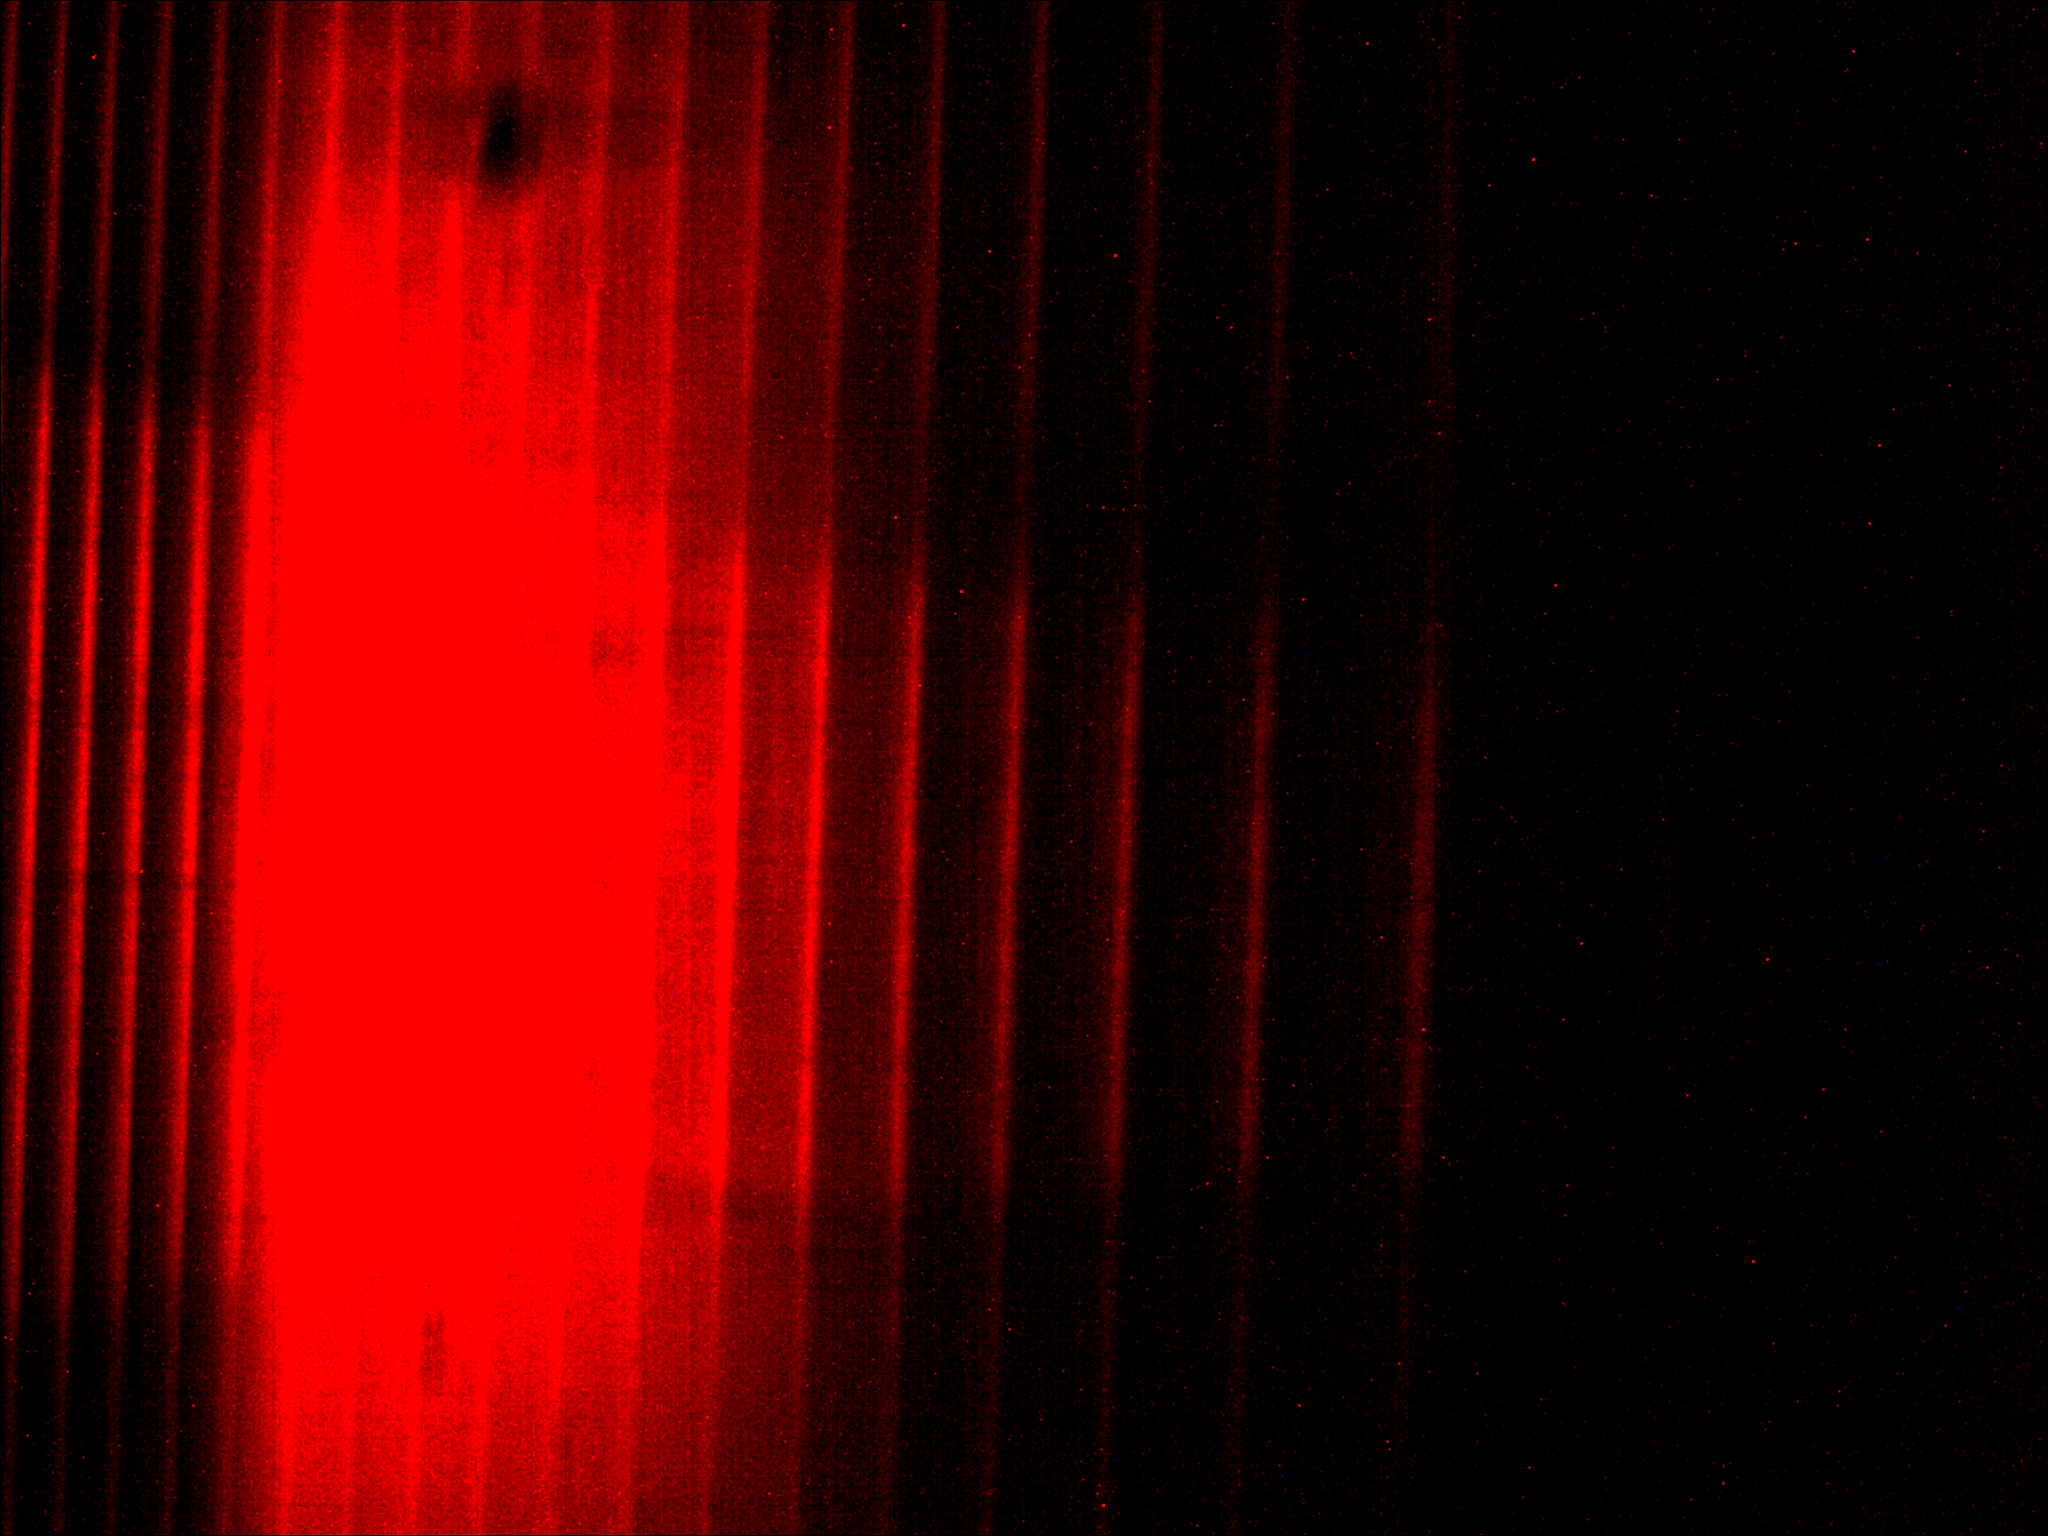
\includegraphics[width=.5\paperwidth, trim={0 0 0 886pt}, clip]{img/long_1}
            \caption{Beobachtete Linien in longitudinaler Richtung, mit $\lambda$/4-Filter und linearem Polarisationsfilter}
            \label{long_mit}
          }
        \end{figure}
      \end{myframe}

      \subsubsection{transversal}
        \begin{myframe}{\subsecname\ - \subsubsecname}
           \begin{itemize}
             \item Beobachtung von 3 Linien
             \item[$\rightarrow$] Rotation des Linearfilters um 90° wechselt zwischen den $\sigma$-Linien und der $\pi$-Linie
             \item[$\rightarrow$] linear polarisiert
           \end{itemize}
        \end{myframe}

        \begin{myframe}{\subsecname\ - \subsubsecname}
          \begin{figure}
            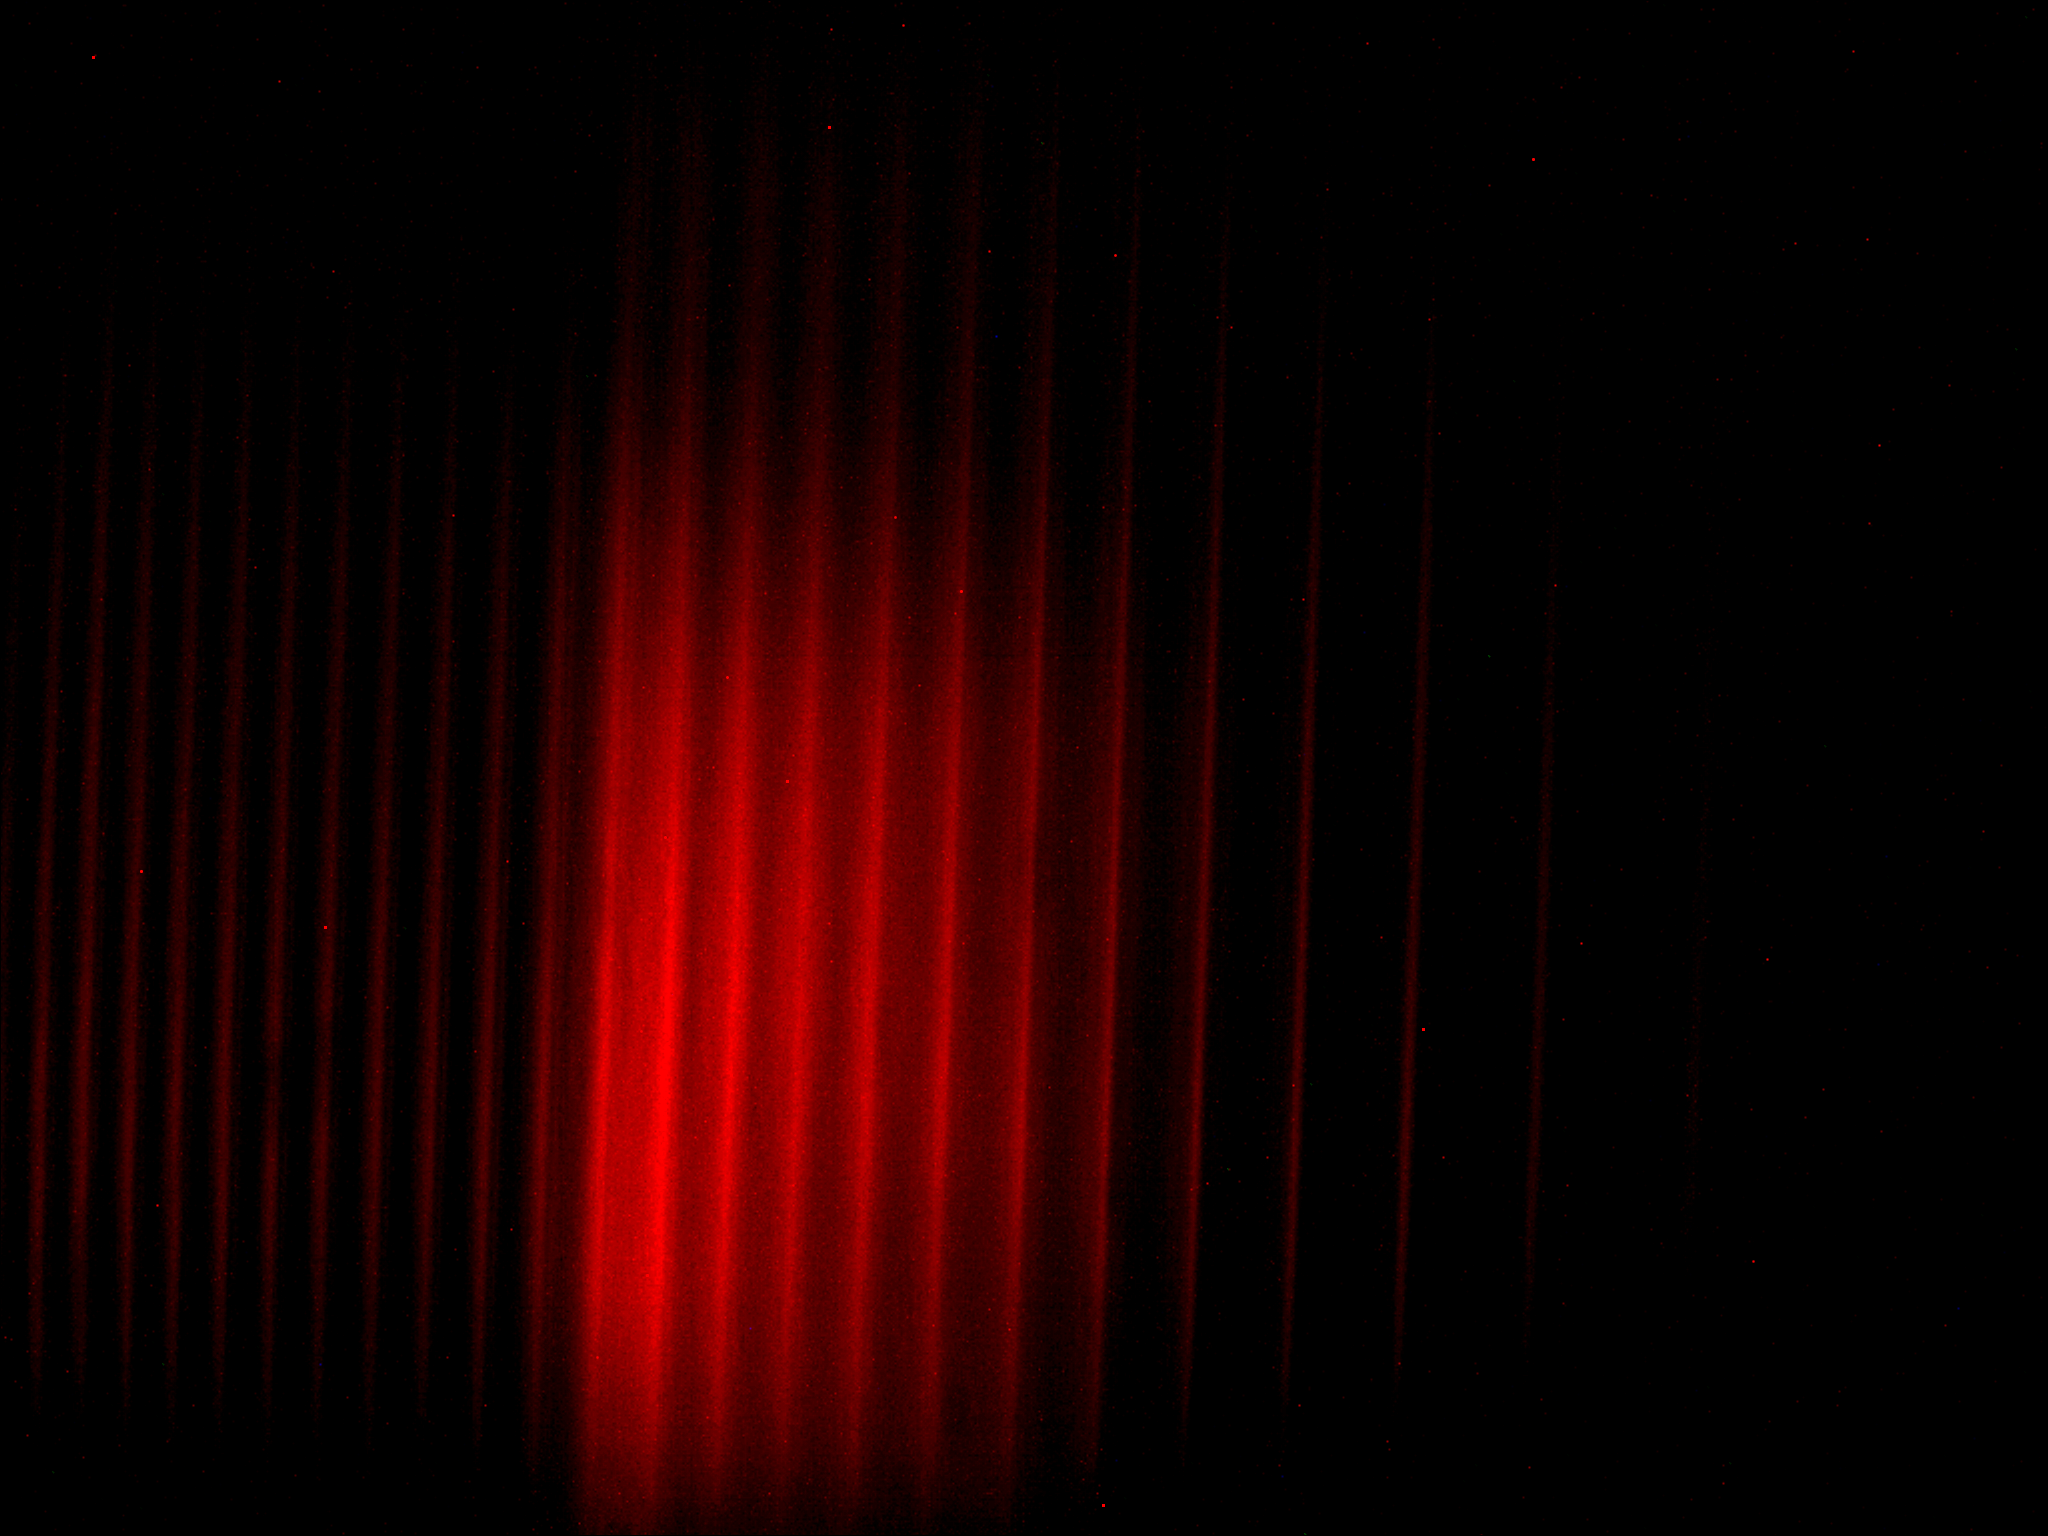
\includegraphics[width=.8\paperwidth, trim={0 300pt 0 900pt}, clip]{img/trans_pi}
            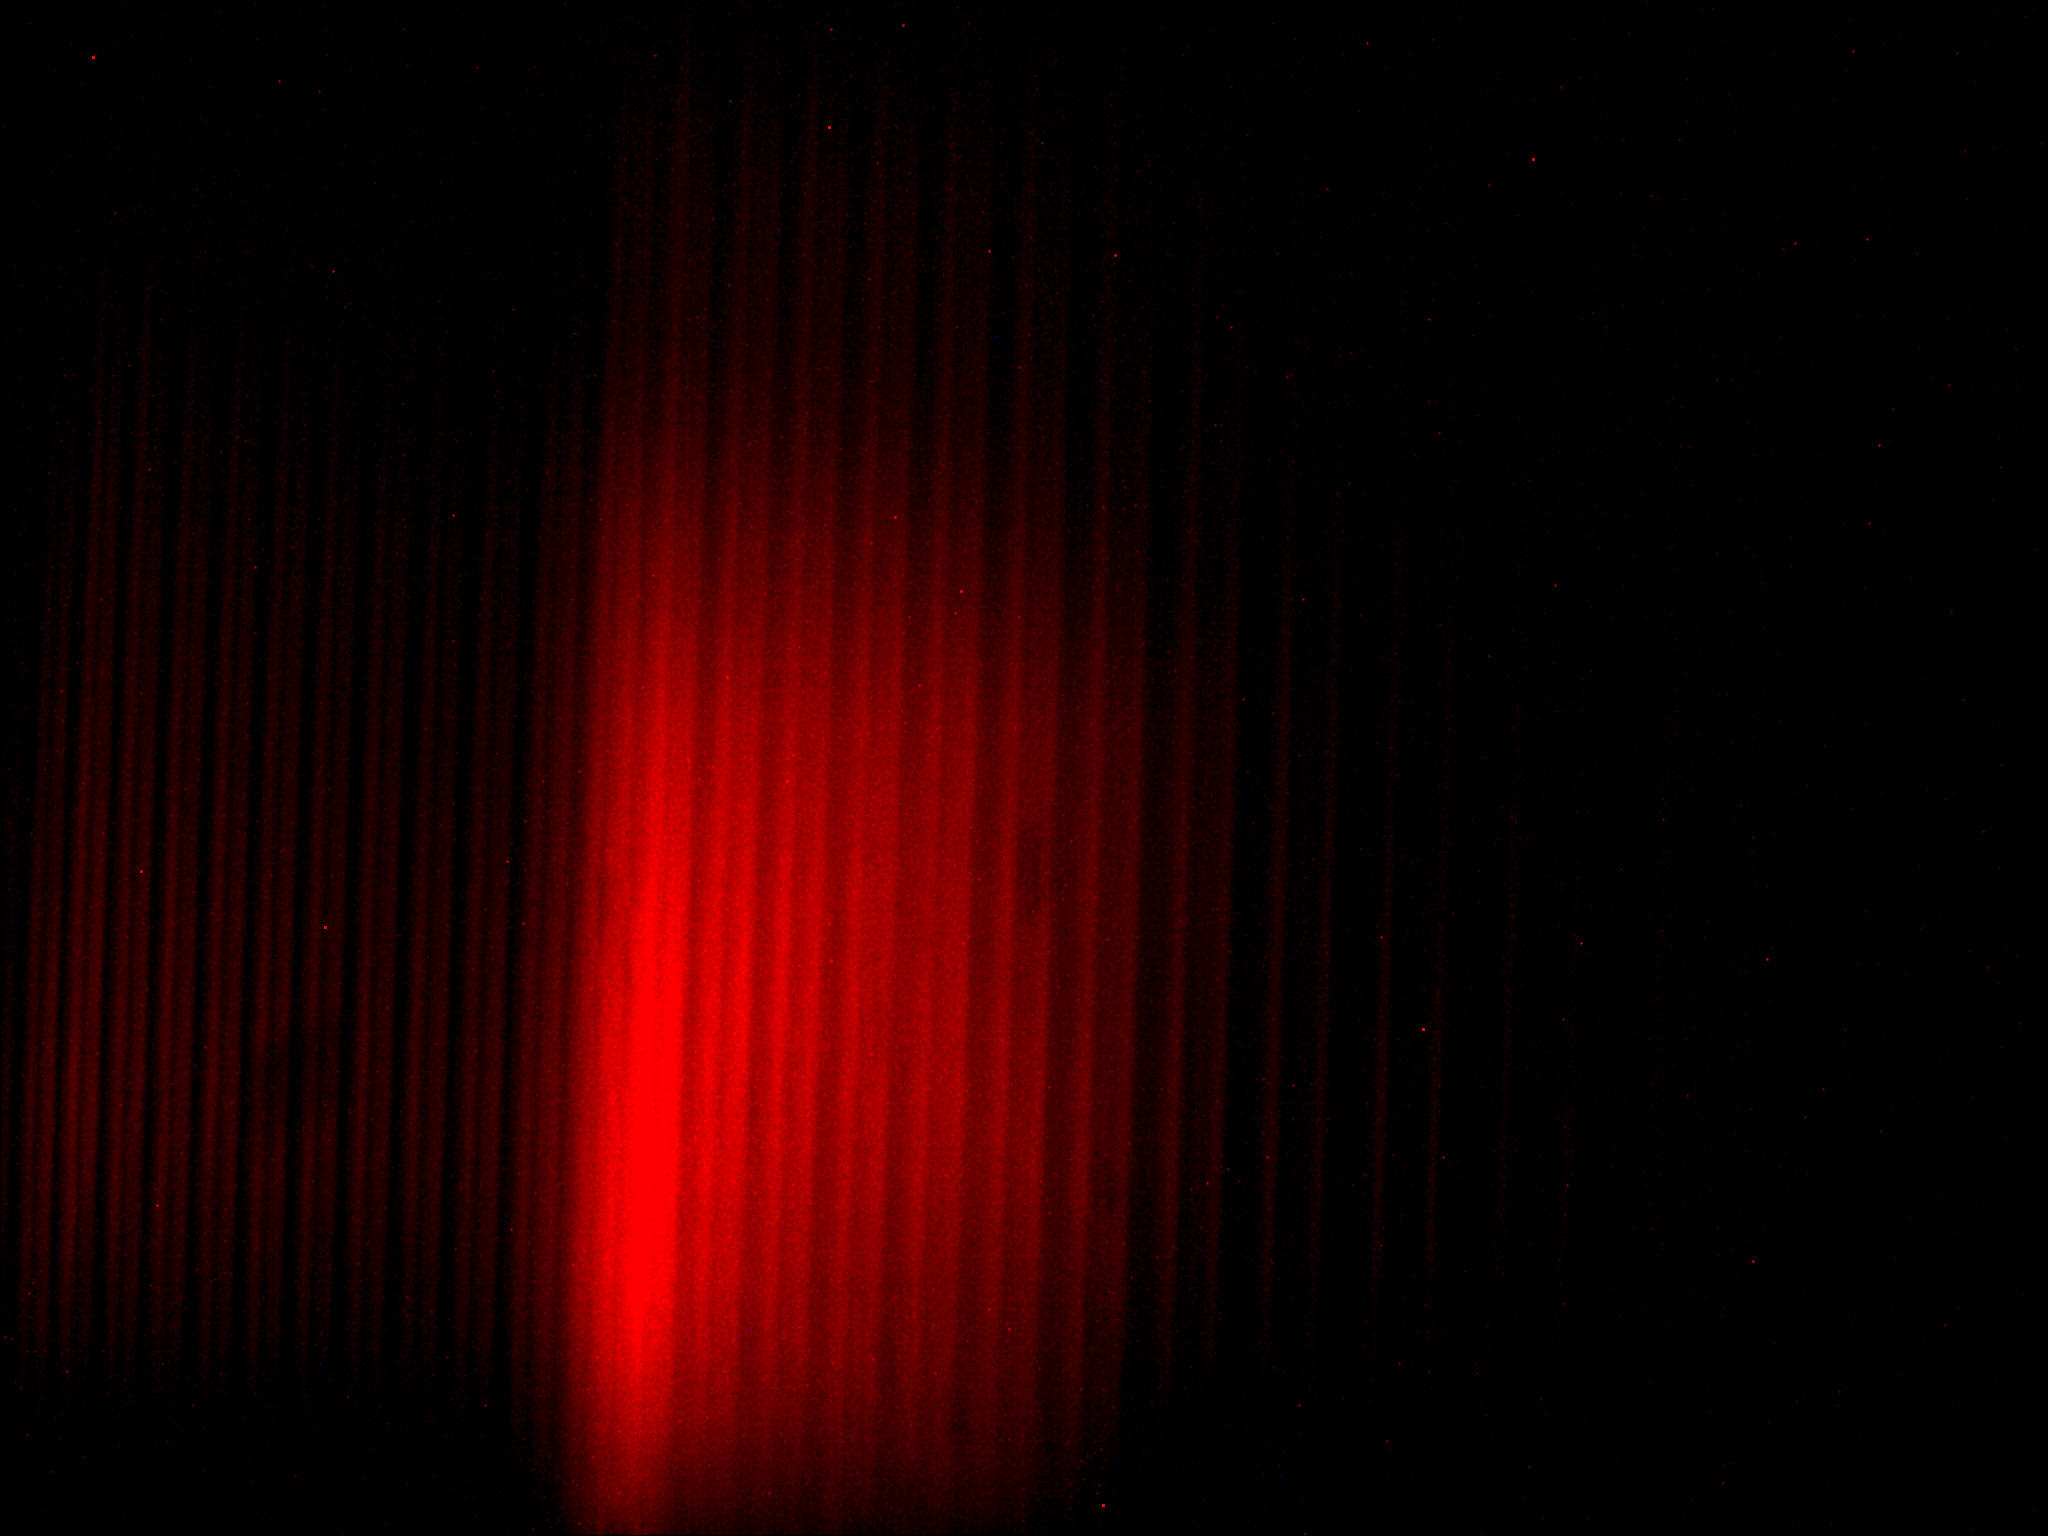
\includegraphics[width=.8\paperwidth, trim={0 300pt 0 900pt}, clip]{img/trans_sig}
            \caption{Beobachtete Linien in transversaler Ausrichtung, mit linearem Polarisationsfilter}
            \label{trans}
          \end{figure}
        \end{myframe}

  \subsection{Bestimmung der Wellenlängenverschiebung}
    \subsubsection{Positionsbestimmung}
      \begin{myframe}{\subsecname\ - \subsubsecname}
        \begin{itemize}
            \item Bestimmung der px-Position von $\sigma$- und $\pi$-Linien
            \item 5 Ordungen
            \item Fit der Peaks für Position und Fehler
            %TODO: input single! pic of pos diagram
        \end{itemize}
      \end{myframe}

    \subsubsection{Ordnungsverschiebung}
      \begin{myframe}{\subsecname\ - \subsubsecname}
        Zuordung
        \begin{tabular}{p{0.48\textwidth}p{0.4\textwidth}}
          \begin{itemize}
            \item (theoretische) ganzzahligen Ordnung
            \item kontinuierliche Polynomfitfkt
          \end{itemize} &
          \begin{itemize}
            \item[] $\mapsto \pi$-linien
            \item[] $\mapsto \sigma$-Linien
          \end{itemize} \\
        \end{tabular}
        %TODO: insert fig 10
        $\Rightarrow$ beobachtete Verschiebung der Beugungsordnung zwischen drei Peaks
      \end{myframe}

    \subsubsection{Wellenlängenverschiebung}
      \begin{myframe}{\subsecname\ - \subsubsecname}
        für kleine Verschiebungen gilt:
        \begin{align}
          \delta\lambda = \frac{\delta a}{\Delta a}\cdot \Delta\lambda\approx\delta k\cdot\lambda k,
          &\qquad\Delta\lambda = \frac{\lambda^2}{2d\cdot\sqrt{n^2-1}}\\
        \end{align}
        \scriptsize (n = \SI{1.4567}{}, d=\SI{4.04e-3}{m})
      \end{myframe}
  \subsection{Bestimmung des Bohr'schen Magneton}
